\subsection{Etapa diferencial} 

En primer lugar identificamos la etapa diferencial en el diagrama del amplificador multietapas, la cual es la que contiene a los transistores $Q_1$ y$Q_2$. Dicha etapa se muestra en la figura \ref{fig:met-etapa-amplificador-de-diferencial}.

\begin{figure}[ht]
    \centering
    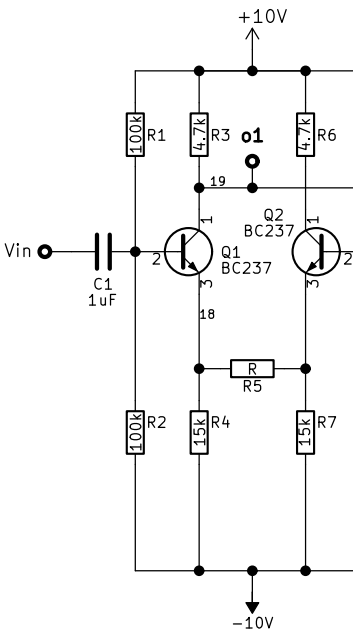
\includegraphics[width=0.33\textwidth]{src/images/metodología/etapa-diferencial.png}
    \caption{Etapa diferencial del amplificador}
    \label{fig:met-etapa-amplificador-de-diferencial}
\end{figure}

Ahora procedemos a calcular los puntos estáticos de operación, para ello tomamos los capacitores como circuitos abiertos, ya que estamos trabajando en DC y empezamos a calcular las corrientes en los transistores.

Asumiremos que la corriente que pasa por $R5$ es 0.

Para calcular la corriente de base se usará el teorema de thevenim para sustituir $R_1$ y $R_2$ por una fuente y una resistencia que pasa por la base de $Q_1$.

Para calcular el valor de la resistencia equivalente de thevenim:
$$R_{th} = R_1 // R_2$$

cómo $R_1 = R_2$
$$Rth = \frac{R_1}{2} = 50k \Omega$$

Ahora, calculamos el valor de la fuente de thevenim aplicando un divisor de voltaje:

$$V_{th} = \frac{R_2 ( V_{cc} - V_{EE}}{R_1 + R_2}$$

$$V_{th} = 10 V$$

Ahora aplicando LVK en la malla B-E ($Q_4$):
\begin{equation*}
V_{th} - R_{th}I_b - V_{be} - R_7(I_e) = 0
\end{equation*}

despejando $I_b$, tenemos

$$I_b = \frac{V_{th} - V_{be}}{R_{th} + (\beta + 1) R_7}$$

usando un $\beta = 230$ entonces

$$I_{b} = 2,65\mu A$$

Ahora, para calcular $I_c$:

$$I_{c} = \beta I_b = 0,62mA$$

Y por último, para calcular $V_{ce}$ aplicamos LVK:

$$Vcc - I_cR_3 - I_eR_4 - V_{ce} - V_{ee} = 0$$

Despejando $V_{ce}$ y aproximando $I_c \approx I_e$, tenemos 

$$V_{ce} = V_{cc}  - V_{ee} - I_c (R_4 + R_3)$$

$$V_{ce} = 7,79 V$$

Como el circuito es simétrico, los voltajes y corrientes $I_b$, $I_e$, $I_c$, $V_{ce}$ y $V_{be}$ son iguales.

El resumén de los puntos estáticos de operación en la etapa diferencial se muestra en la tabla \ref{tab:amplificador-diferencial-puntos-estaticos}.

\begin{table}[ht]
    \centering
    \begin{tabular}{|c|c|c|}
        \hline
        Transistor & \textbf{$I_c$} & \textbf{$V_{ce}$} \\
        \hline
        $Q_1$ & $0,62 mA$ & $7.79 V$ \\
        $Q_2$ & $0,62 mA$ & $7.79 V$ \\
        \hline
    \end{tabular}
    \caption{Puntos estáticos de operación en la etapa diferencial}
    \label{tab:amplificador-diferencial-puntos-estaticos}
\end{table}

Ahora, para la parte dinámica, calculamos los parámetros del transistor utilizando $V_t = 26 mV$ y $V_A = 100 V$

$$gm = \frac{I_c}{V_t} = \frac{0,62 mA}{26 mV}$$

$$gm = 23,85 \times 10 ^{-3}$$

$$R_\pi = \frac{\beta}{gm} = \frac{230}{23,85\times 10^{-3}}$$

$$ R_\pi = 9,6k \Omega$$

$$ R_o = \frac{V_A}{I_c} = \frac{100 V}{0,62 mA} = 161,29 k\Omega$$

Resumimos los parámetros dinámicos de los transistores de la etapa diferencial en la tabla \ref{tab:met-etapa-diferencial-parametros-dinamicos}.

\begin{table}[ht]
    \centering
    \begin{tabular}{|c|c|c|c|}
        \hline
        Transistor & $R_\pi$ & $gm$ & $R_o$ \\
        \hline
        $Q_1$ & $9.6 k\Omega$ & $23.85mS$ & $161.29k\Omega$ \\
        \hline
        $Q_2$ & $9.6 k\Omega$ & $23.85mS$ & $161.29k\Omega$ \\
        \hline
    \end{tabular}
    \caption{Parámetros dinámicos de los transistores de la etapa diferencial}
    \label{tab:met-etapa-diferencial-parametros-dinamicos}
    \end{table}

Tomando el amplificador en su modo común, en primer lugar calculamos la impedancia de entrada, analizando el circuito obtenemos la expresión:

$$ Z_c = R_1 || R_2 || (R_\pi + (1 + gmR_\pi)R_4)$$

sustituyendo los valores tenemos:

$$ Z_c = 49K\Omega$$

Ahora la impedancia de salida es:

$$ Z_o = Z_{cc} \parallel r_3$$

donde

$$ Z_{ccQ1} = \frac{r_\pi + r_1/2 + [(1 + gmr_\pi) + \frac{r_\pi + r_1/2}{R_o}] r_4}{\frac{r_\pi + r_1/2 + r_4}{r_o}}$$

$$ Z_{ccQ1} = 7.63 M\Omega$$

pero, como $Z_{ccQ1} >> r_3$ entonces:

$$ Z_0 = r_3 = 4.7k\Omega$$

Ahora la ganancia es:

$$A_c = - \frac{ gmR_\pi R_3}{R_\pi + (1 + gmR_\pi)R_4}$$

$$A_c = 0,31$$

Ahora analizamos en modo diferencial:

$$Z_d = R_1 || R_2 || (2R_\pi + (1+gmR_\pi )R_5)$$

$$Z_d = 43,99 k\Omega$$

$Z_o$ es la misma que en modo común:

$$Z_0 = 4,9 K\Omega$$

Por último calculamos la ganancia en modo diferencial:

$$A_d = -\frac{gmR_\pi R_3}{2R_\pi + (1 + gmR_\pi) R_5}$$

$$A_d = -2,96 $$

Los datos del modelo dinámico de la etapa diferencial se muestran en la tabla \ref{tab:met-etapa-diferencial-modelo-dinamico-modo-comun} para el modo común y en la tabla \ref{tab:met-etapa-diferencial-modelo-dinamico-modo-diferencial} para el modo diferencial.

\begin{table}[ht]
    \centering
    \begin{tabular}{|c|c|}
        \hline
        parámetro & valor  \\
        \hline
        $Z_i$ & $49k\Omega$ \\
        \hline
        $Z_o$ & $4.7k\Omega$ \\
        \hline
        $A$ & $0,31$ \\
        \hline
    \end{tabular}
    \caption{Modelo dinámico de la etapa diferencial modo común}
    \label{tab:met-etapa-diferencial-modelo-dinamico-modo-comun}
\end{table}

\begin{table}[ht]
    \centering
    \begin{tabular}{|c|c|c|}
        \hline
        parámetro & valor  \\
        \hline
        $Z_i$ & $43,99k\Omega$ \\
        \hline
        $Z_o$ & $4.7k\Omega$ \\
        \hline
        $A$ & $-2,96$ \\
        \hline
    \end{tabular}
    \caption{Modelo dinámico de la etapa diferencial modo diferencial}
    \label{tab:met-etapa-diferencial-modelo-dinamico-modo-diferencial}
\end{table}

\begin{figure}[ht]
    \centering
    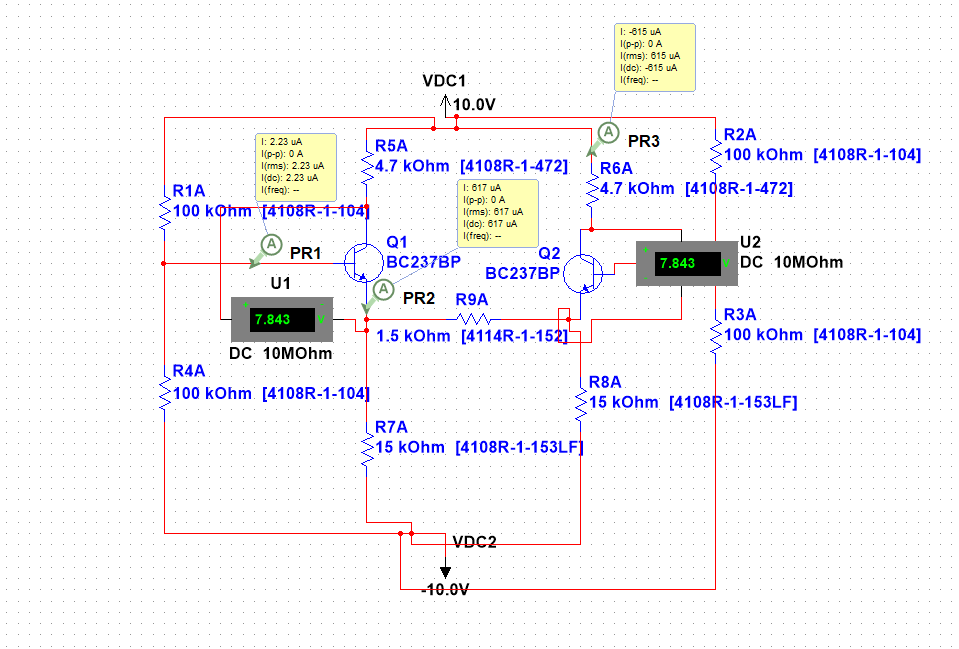
\includegraphics[width=0.9\textwidth]{src/images/p2/punto-estatico-p2.png}
    \caption{Simulación puntos estáticos etapa diferencial}
    \label{fig:sim-etapa-diferencial-puntos-estaticos}
\end{figure}

\begin{figure}[ht]
    \centering
    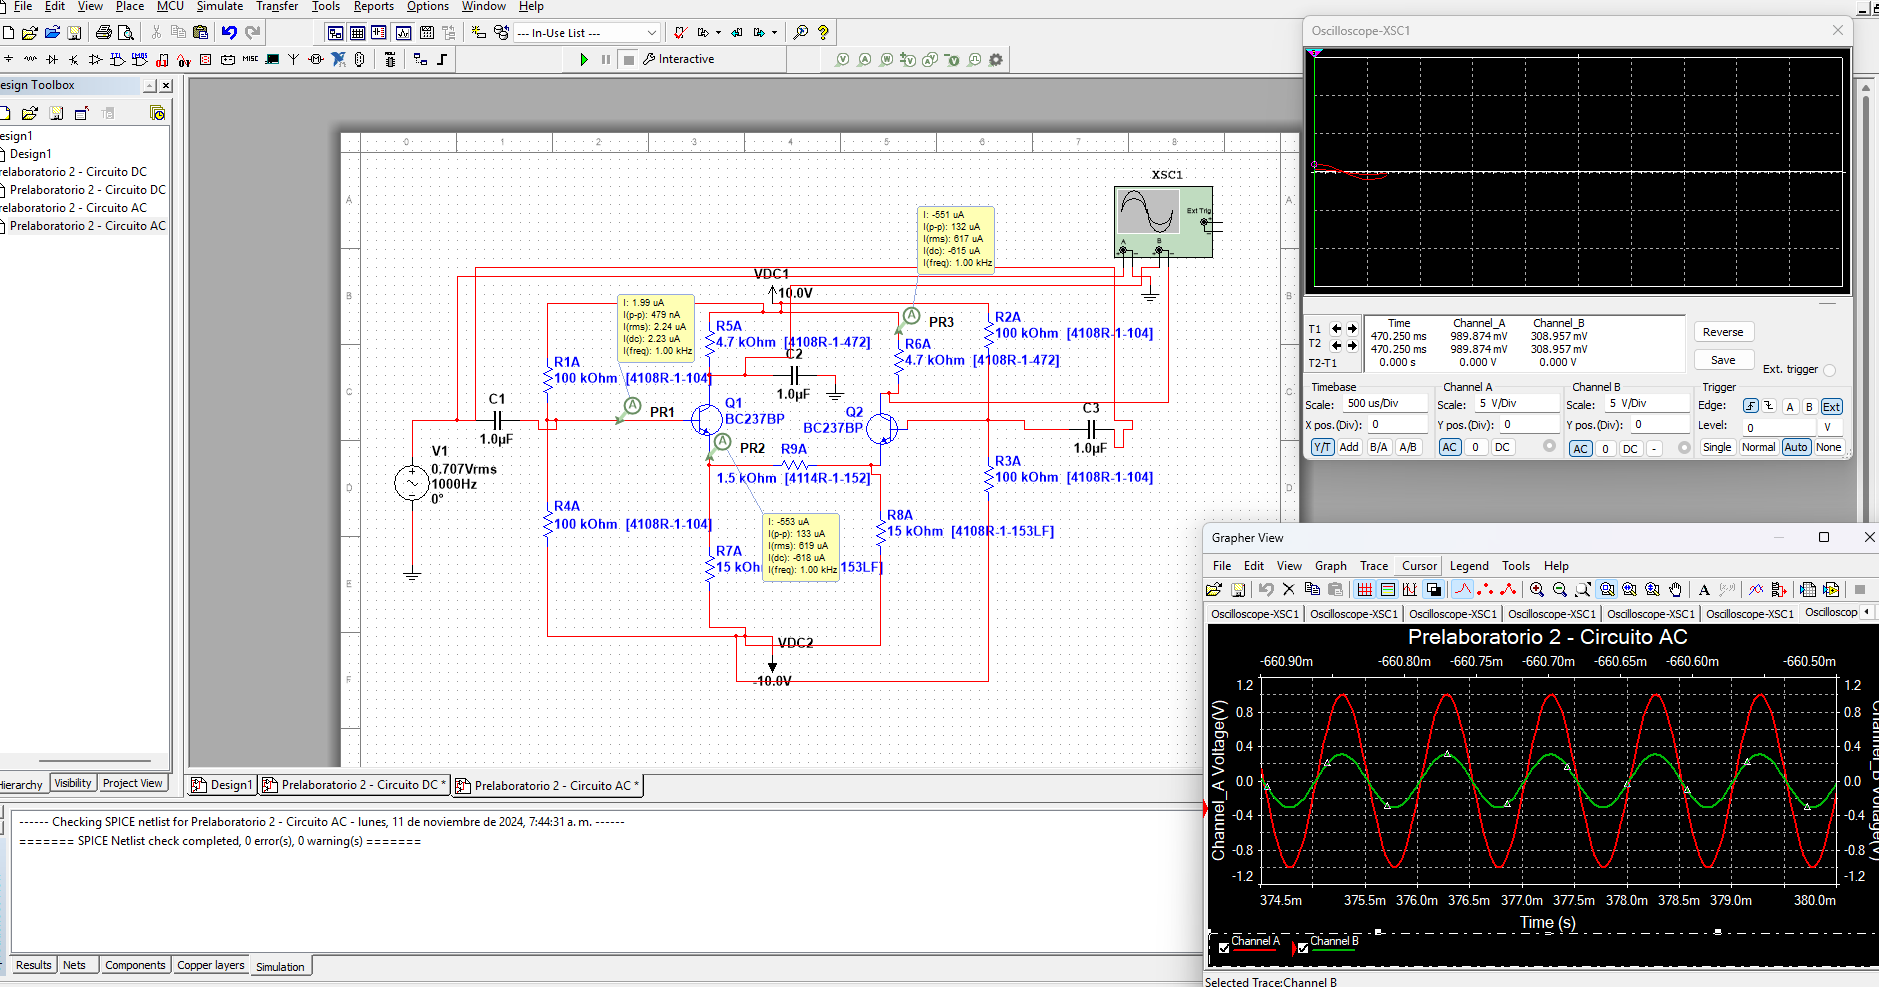
\includegraphics[width=0.9\textwidth]{src/images/p2/ganancia-etapa-diff-modo-comun.png}
    \caption{Simulación ganancia etapa diferencial modo común}
    \label{fig:sim-etapa-diferencial-ganancia-modo-comun}
\end{figure}

\begin{figure}[ht]
    \centering
    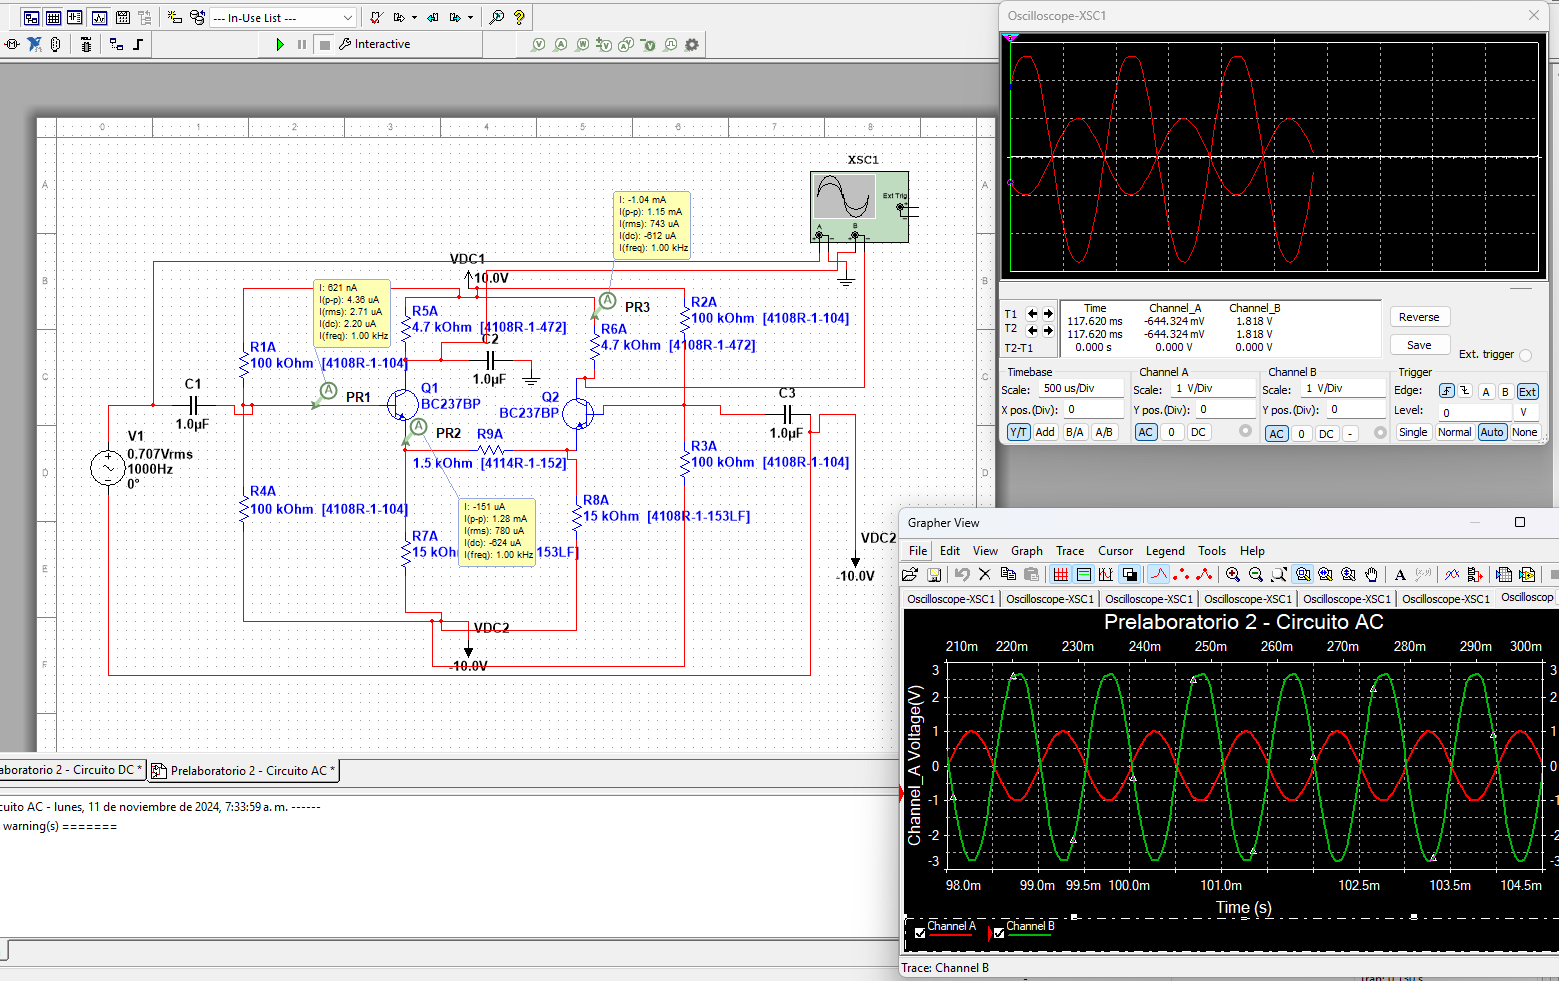
\includegraphics[width=0.9\textwidth]{src/images/p2/ganancia-etapa-diff-modo-diff.png}
    \caption{Simulación ganancia etapa diferencial modo diferencial}
    \label{fig:sim-etapa-diferencial-ganancia-modo-diferencial}
\end{figure}


\begin{table}[ht]
    \centering
    \begin{tabular}{|c|c|c|}
        \hline
        Modo & $V_i$ & $\delta V_i$ \\
        \hline
        modo diferencial & $2V$ & $100mV$ \\
        \hline
        modo común & $12.8V$ & $0.4V$ \\
        \hline
    \end{tabular}
    \caption{Límite de máxima excursión}
\end{table}


\begin{figure}[ht]
    \centering
    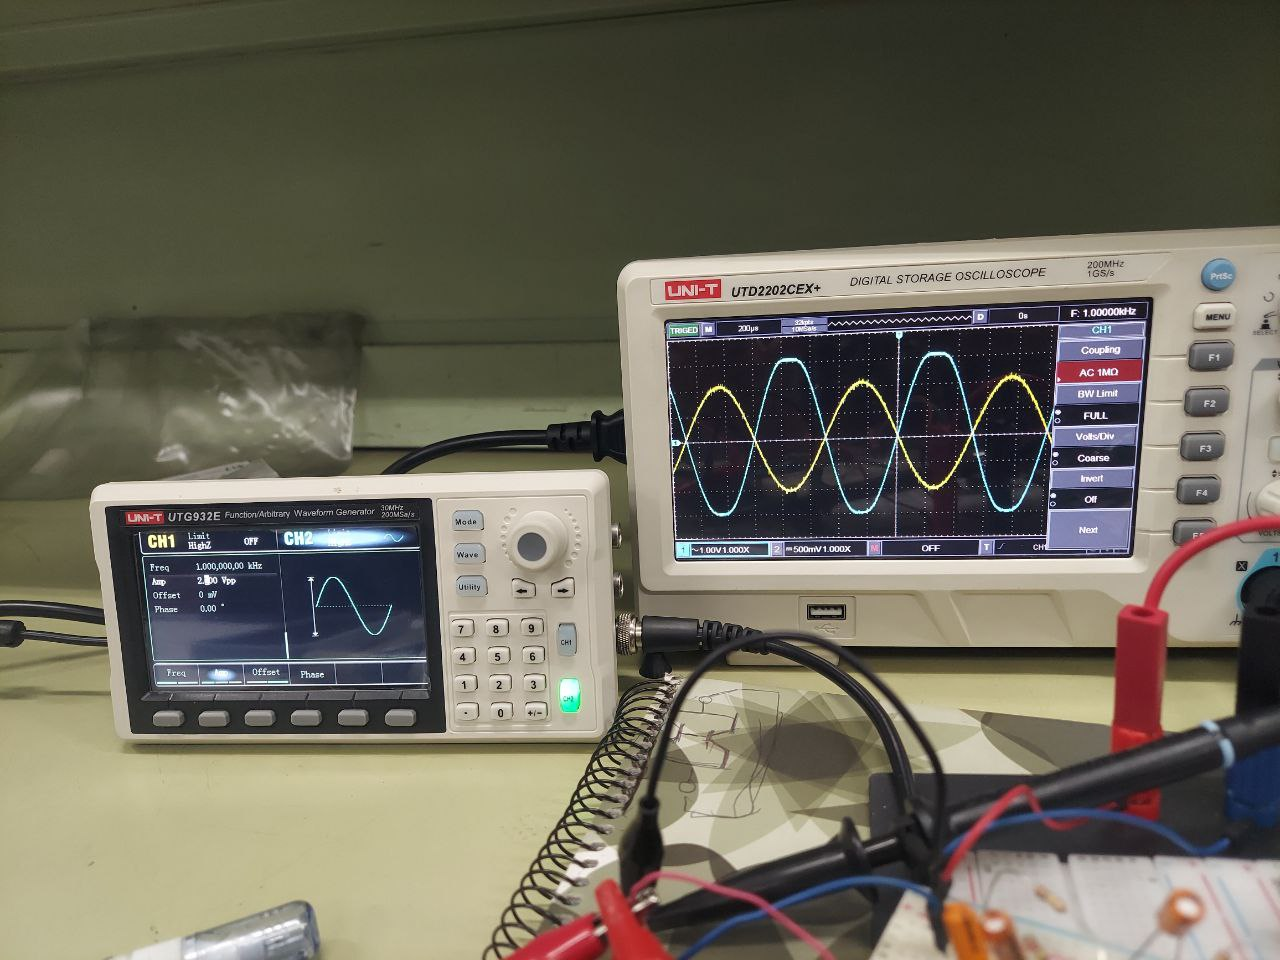
\includegraphics[width=0.5\textwidth]{src/images/p2/limite-excursion-diferencial.jpg}
    \caption{Límite de máxima excursión etapa diferencial modo diferencial}
\end{figure}

